%
% fig-homotopie.tex
%
% (c) 2025 Prof Dr Andreas Müller
%
\begin{figure}
\centering
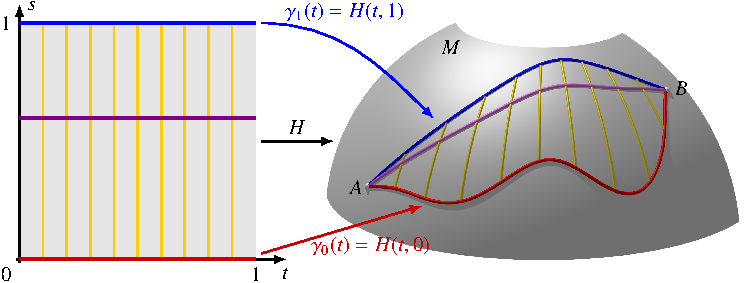
\includegraphics{chapters/040-green/images/homotopie.pdf}
\caption{Eine Homotopie zwischen den beiden Wegen $\gamma_0(t)$
und $\gamma_1(t)$ in der Mannigfaltigkeit ist eine Abbildung
$H\colon [0,1]\times[0,1]\to M$ mit $\gamma_0(t)=H(t,0)$ und
$\gamma_1(t) = H(t,1)$.
\label{buch:green:fig:homotopie}}
\end{figure}
